%%% tfs.tex ---
%% 
%% Version: $Id: tfs.tex,v 0.0 2007/11/12 01:06:14 yzf Exp$
%% Note: coding: utf-8;mode: pdflatex

%\revision$Header: /home/yzf/myWorkspace/tplatform/tfs/dev/paper/tfs.tex,v 0.0 2007/11/12 01:06:14 yzf Exp$
\documentclass[11pt,a4paper]{scrartcl} %KOMA-Script instead of standard class
\usepackage{CJKutf8}
\usepackage{indentfirst}
\usepackage[debugshow,final]{graphics}
\usepackage{url}
\bibliographystyle{acm} % plain,abbrv,alpha,apalike,unsrt,acm,ieeetr,siam
%\frenchspacing % not to insert extra space at the end of sentences
%\pagestyle{headings}
%\addtolength{\hoffset}{-0.5cm}
%\addtolength{\textwidth}{1cm}
\setlength{\parindent}{2em}     % paragraph indent 2 characters
\usepackage[pdftex,bookmarks,unicode,colorlinks,linkcolor=red,citecolor=green,filecolor=magenta,urlcolor=blue]{hyperref}
%%================================================================
%% begin document
%%================================================================
\begin{document}
\begin{CJK*}{UTF8}{gbsn}
\CJKcaption{zh-Hans}
\title{TFS: 天网文件系统}
\author{{\rm 杨志丰,彭波,涂其琛,樊锴,陈日闪,朱磊}\\
\{yzf,pb,tqc,fankai,crs,zhulei\}@net.pku.edu.cn\\
北京大学网络实验室}
\date{}
\maketitle
%\tableofcontents

\subsection*{摘要}
\subsection*{关键字}
\section{介绍}
\subsection{背景}
在Web迅速发展的背景下,以Google为代表的搜索引擎获得了巨大成功。在这样耀眼的成功后面,人们开始意识到,我们已经进入到一个数据为王的时代,谁拥有越多的数据,拥有越强的数据处理能力,谁就有可能够成为技术革新的领跑者。在不断增长的海量Web数据中蕴藏着无数的宝藏,等待人们去发掘,Web信息检索和Web数据挖掘已经成为当前计算机研究工作的热点,而如何为这样的海量数据处理提供高效的计算环境也逐渐成为一个被人们重视的问题。

TFS(TianwangFileSystem)是针对海量数据处理所必需的存储、数据管理服务而设计的一个分布式文件系统。这一项目是由Tianwang系统运行中的实际需求推动而开始的。我们工作中出现的实际问题也是从事海量数据处理的研究和技术人员面临的典型问题,比如硬盘、机器故障导致数据丢失;数据的存储、访问方式需要应用程序来考虑,出现了大量重复低效率的工作;虽然不断增加机器,但机器仍然主要在被独占使用,利用率不高。通过实现一个独立的软件系统来解决这些问题,这样一个工作的重要性越来越高。它是海量数据处理基础设施里的一个中心环节。

\subsection{相关工作}
分布式文件系统研究方向里有大量的优秀工作,具体在海量Web数据处理基础设施的相关工作中,相关工作中最有代表性和开创性的是Google File System\cite{gfs2003}。Google在大量的廉价(易失效)PC和网络连接的硬件平台基础上实现了一个可靠的,高扩展性,高性能的分布式文件系统。在2003的OSDI上发表这一工作的论文后,Google在这个方向上的工作不断深入,相继发表了MapReduce\cite{mapreduce},BigTable系统\cite{bigtable}的论文,也让更多的人从Google的工作中认识到这一工作的重大意义。Google展示了一个超级计算平台的雏形,这一技术成为其公司的核心价值所在。

另一个工作是开源的Hadoop项目\cite{hadoop},它最早是Lucene/Nutch的作者Doug Cutting在Nuctch系统中实现的一个GFS/MapReduce模块,后来独立成为hadoop项目。作为一个活跃的开源项目,它帮助人们从一种实现的角度更加深入的认识这一工作。Hadoop基本沿用GFS的设计思想,但是简化了设计,不支持相对复杂的原子追加,只支持单一写者模型。较新的类似工作,还有KFS\cite{kfs},它是一个C++实现的更加类似GFS的系统,比hadoop支持更多的特性。微软的Dryad\cite{Dryad2007}也表明他们也在这个方向上有相当多的工作,只是目前还没有公开的文件系统的论文。

我们把构建海量数据处理的基础设施作为目标,TFS是我们在这一方向上努力的开始。
\section{设计概述}
Tianwang文件系统的体系结构和Google文件系统基本一致。一个文件由若干个文件块组成,每个文件块是存储在某个数据节点上的普通文件。每个文件块都有若干个副本。系统由三种角色共同构成。一个master节点,用来存储文件系统的原数据。若干个chunkserver节点,用来存储实际构成文件的数据。若干个client节点通过和master、chunkserver的通讯来进行读写等文件系统的操作。
\subsection{块大小}
在Google文件系统中,每个文件块的大小都是固定的(64M)。在原有的读写语义下,为了保证每个数据块的大小一致,当要追加的数据大小大于当前块可以容纳的数据大小的时候,系统会把这个块填充满,然后把数据写入到下一个块。当写失败的时候,系统会指示客户端从一个新的位置重新执行写操作。这样,同一个文件块的多个副本在内容上不完全一致,并且可能存在不完整的数据片断,需要读取数据的应用程序做出更多的努力。

而在我们Tianwang文件系统里,组成一个文件的不同文件块的大小是不同的。也就是说,系统中文件块的大小是不定长度的。结合我们特有的写操作的语义(见下面各节),我们的系统中不会出现填充、数据片断和不一致的数据。当然,这种改进带来了其他方面的开销,比如,我们的每个文件块数据结构要带一个长度属性,这增加了内存开销。但是我们的关键的读操作和记录追加操作的性能并没有下降。
\subsection{读操作}
在一次读操作中,client通过与master的通讯得到要读的文件块的位置,然后与相应的chunkserver通讯,读取数据。这一过程也因为块大小是否可变的不同决策而导致不同。

在使用固定的块大小的Google文件系统中,client通过计算把文件内字节偏移转换为文件中的块序号。然后,他把文件名和块序号发送给master,master返回对应的块标识和存储位置。client缓存这些信息,并选择一个最近的包含该块的chunkserver,发送块标识和块内的一块字节区域给chunkserver,然后chunkserver把数据发送给client。client端缓存的元数据在一定时间之后失效。

在我们的系统中,因为块大小不同,客户端无法把一个偏移量之间转换为块序号。他必须知道组成文件的所有块的大小,才能决定要读的是哪个文件块。所以,当客户端以读方式打开一个文件的时候,他从master得到组成这个文件的所有文件块以及他们的存储位置信息。读的时候通过计算找到相应的块,然后和相应的chunkserver进行通讯读取数据。这样做虽然是由文件块大小不同这个客观属性决定的,但它的优点是,对一个文件的一系列读操作只需要与master进行一次通讯,而原有的设计,每次读一个新的块都需要进行一次与master的通讯,在缓存的元数据失效之后,可能进行更多次的通讯。不过,这样做的缺点是,在一个客户端打开一个文件之后,如果有其他客户端对这个文件追加了数据,这些数据对这个客户端是不可见的。但是,考虑到我们的追加操作在绝大多数情况下都是一次性完成的,我们认为这样的缺点也是可以接受的。如果在某些应用下,这一问题变的很关键时,改进也非常简单:可以对块数据增设一个失效时间,在失效之后和master重新进行一次通讯,这样,数据的时新性就是可控的了。
\subsection{记录写}
系统设计决策的一个重要目标是支持多个client并发的对同一个文件进行高效的追加操作。

在Google文件系统中,使用租约(lease)机制来保证对一个块的多个复本修改操作(包括记录追加和写操作)的执行顺序(见~\cite{gfs2003}~3.1节)。当要写一个文件块的位于多个chunkserver的多个副本时,其中一个chunkserver扮演与其他的chunkserver不同的角色,它是对这个块的所有修改操作的顺序的控制者(我们把它叫做“主chunkserver”),其他副本依照和他同样的顺序实施修改操作。

在google文件系统中,当你追加一个记录到文件时,主chunkserver判断当前最后一个文件块是否有足够的剩余空间容纳数据,如果可以,就写入这个块,否则,系统把当前文件块填充,然后指示客户端写入下一个块。当一个副本写失败的时候,客户端重试追加操作,这一操作是从某个文件块所有副本的一个新的位置开始写入。所以,对于应用程序来说,追加操作成功的语义是,数据至少被完整的写入文件一次。在操作成功的区域内,数据是在各个复本上是一致,并且数据是完整的。但是在不成功的区域中,数据在各个复本上是不一致的。所以,Google文件系统中用记录追加方式生成的文件中,记录可能有重复,有不完整的片断,并且可能有系统填充的空白。

\begin{figure}
  \centering
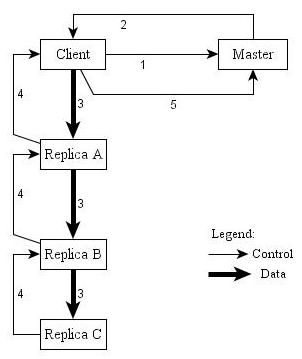
\includegraphics{tfs_write}  
  \caption{TFS记录追加操作}
  \label{fig:tfswrite}
\end{figure}
在我们的系统中,没有使用复杂的租约机制。追加操作已文件块为单位,如图\ref{fig:tfswrite}所示。交互步骤如下:
\begin{enumerate}
\item 客户端向master申请一个新的文件块用于追加数据。
\item master分配一个新的块,并根据当前各个chunkserver的负载从中选择若干个返回给客户端,用于客户端写入数据。
\item 客户端把数据和写入命令发送给距离他最近的chunkserver,第一个chunkserver再把数据和写入命令发送给下一个chunkserver,以此类推,系统用流水线的方式完成数据传输。
\item 系统把每个chunkserver写数据成功与否的消息以流水的方式传回给客户端。
\item 如果至少有一个chunkserver的数据写成功了,客户端通知master写成功,并把写成功的chunkserver告诉master,master会把这些信息记录在自己的内部数据结构中,并标记这个块为文件的一个块。如果没有一个chunkserver的数据写成功,客户端可以重试若干次,如果还是失败,客户端通知master丢弃这个块,然后把错误递交给应用程序处理。
\end{enumerate}
所以,每一个文件块只有一个客户端在写入,我们的系统通过允许一个文件在同一个时刻有多个块被追加来实现了并发的追加。但是,并不是应用程序每追加一条记录就会产生一个新的文件块,系统的客户端库把多次追加操作的数据缓存下来,当达到指定块大小的时候,才进行一次前面所述的交互过程产生一个文件块。在客户端出现异常情况的时候,可能有部分被追加的数据没有写入到系统而丢失。如果有的应用不能容忍这种可能的情况,我们给应用程序提供了flush操作来保证每次追加的数据都写入了系统。

\subsection{写操作}
在Google文件系统中,普通写操作采用与记录追加同样的租约机制。此时,并发的写操作是允许的,但是结果是不确定的(被并发写的区域很可能的结果是多个写操作的片段的集合)。但是只要写操作成功了,租约机制保证了多个复本内容是一致的(即使内容不是所期望的)。

我们认为,Google文件系统为了实现并发的写操作而采用复杂的租约机制是得不偿失的。在提供了记录追加的情况下,写操作主要是重写操作(重写已有数据块的一段区域)。首先,花了巨大的功夫,并发写产生的结果虽然是一致的,但却是无用的。其次,并发的重写操作是非常罕见的。因为记录追加和普通写采用了同样的租约的流程,这一流程主要是为了保证重写操作的一致性语义,追加操作实际上是迁就了重写操作。为了迁就一个罕见的操作而放弃了进一步提高一个需要高效实现的操作的性能的可能,我们认为是不明智的。

在Tianwang文件系统中,写操作和记录追加操作是严格区别开的。当一个客户端以写方式打开一个文件时,我们会给该文件加上写锁,所以,写操作不允许并发。而追加操作给文件上的是读锁,读锁允许并发。
\subsection{应用程序的约定}
我们假设通常的应用模式是这样的。多个程序作为“写者”同时向一个文件追加数据,产生一个大文件。然后多个应用程序顺序读取这个文件的数据,进行处理,结果追加到一个新的文件中。

对于能表示为某种记录格式的数据,应用程序最好通过记录追加写而不是普通写操作来添加数据。这不仅是因为普通写操作不支持并发,而且,即使在一个写者的情况下,记录追加的方式也更高效。使用记录追加写的应用,如果可以接受延迟写可能产生的数据丢失(实际上,对于大规模Web数据处理,这个假设是很合情合理的),最好不使用系统提供的flush操作。


在我们的系统中,因为块大小可变,所以系统不会自动在被追加数据的文件中添充空白。我们的追加写是以块为单位的写,所以被成功追加的数据,在文件中是必然完整的存在唯一一份(exactly-once),而不是像Google文件系统中一样,数据可能被写入多次(at-least-once语义)。所以我们的追加操作也不会产生重复的数据和不完整的数据。在Google文件系统中,为了处理空白和不完整的数据,要求应用程序写入的数据自己带有校验和,在读取的时候通过校验和来识别错误的数据。而且,为了处理可能重复的数据,被写入的每条记录都要有全局唯一的标识,读取的时候通过这个标识来去除重复。而我们知道,在分布式大规模数据处理中,产生全局唯一的标识本身就是一个比较困难的任务。所以,我们的系统不要求记录自带全局唯一的标识和校验和。

但是,Tianwang文件系统与Google文件系统一样,不保证并发写入的不同块之间的顺序。一个应用程序的两次连续的追加操作,最终可能产生的文件块(在读取文件时)在逻辑上并不相邻。所以,我们说追加操作是“记录”的,这意味着应用程序关心的是每条数据本身的完整性,而不关心他们在文件中处于什么位置。

\section{实验}

\section{结论}

\bibliography{myBib} % my bibliography database
\end{CJK*}
\end{document}

%%% Local Variables: 
%%% mode: latex
%%% TeX-master: t
%%% End: 
